\section{Results}
\label{sec:exp}

Hill climbing produces excellent results on most networks.  Table ~\ref{table:errors} shows the improvements in the error after running hill climbing for 24 hours.

Although performance varies across networks, we get at least a 50\% decrease in error for all networks except aut-as19990628 and cit-scimet.  For some networks we get an enormous reduction in error; pwr-power gives a 99.5\% reduction and met-HI gives a 99.9\% reduction.  The first group of figures plots the reduction in error over time and the second group plots the probability that a rewiring step will be successful (i.e. that we will accept the changes instead of discarding them).

\begin{table*}[t]
\begin{tabular}{| l | l | l | | l | l | l |}
\hline
Network & Nodes & Edges & Initial error & Final error & Successful rewires\\ \hline
aut-as19971108 & 3015 & 5156 & 0.34216 & 0.16717 & 2951.00\\\hline
aut-as19990628 & 5322 & 10163 & 0.31571 & 0.17723 & 3397.28\\\hline
cit-scimet & 3085 & 13474 & 0.83063 & 0.73247 & 1921.71\\\hline
col-ca-GrQc & 5242 & 14484 & 2.05549 & 0.93973 & 40583.8\\\hline
col-netscience & 1461 & 2742 & 3.13864 & 0.55110 & 8290.71\\\hline
met-HI & 1424 & 3423 & 8039.58 & 0.46768 & 5703.57\\\hline
ppi-ppiall & 3258 & 12930 & 1.06249 & 0.46058 & 38131.1\\\hline
ppi-ppiapms & 1622 & 9070 & 1.37580 & 0.54219 & 24581.7\\\hline
pwr-power & 4941 & 6594 & 0.57996 & 0.00282 & 9485.4\\\hline
\end{tabular}
\caption{Improvements in error after running hill climbing for 24 hours.  All numbers are averaged over $7$ trials.}
\label{table:errors}
\end{table*}

\begin{figure}[p]
\centering
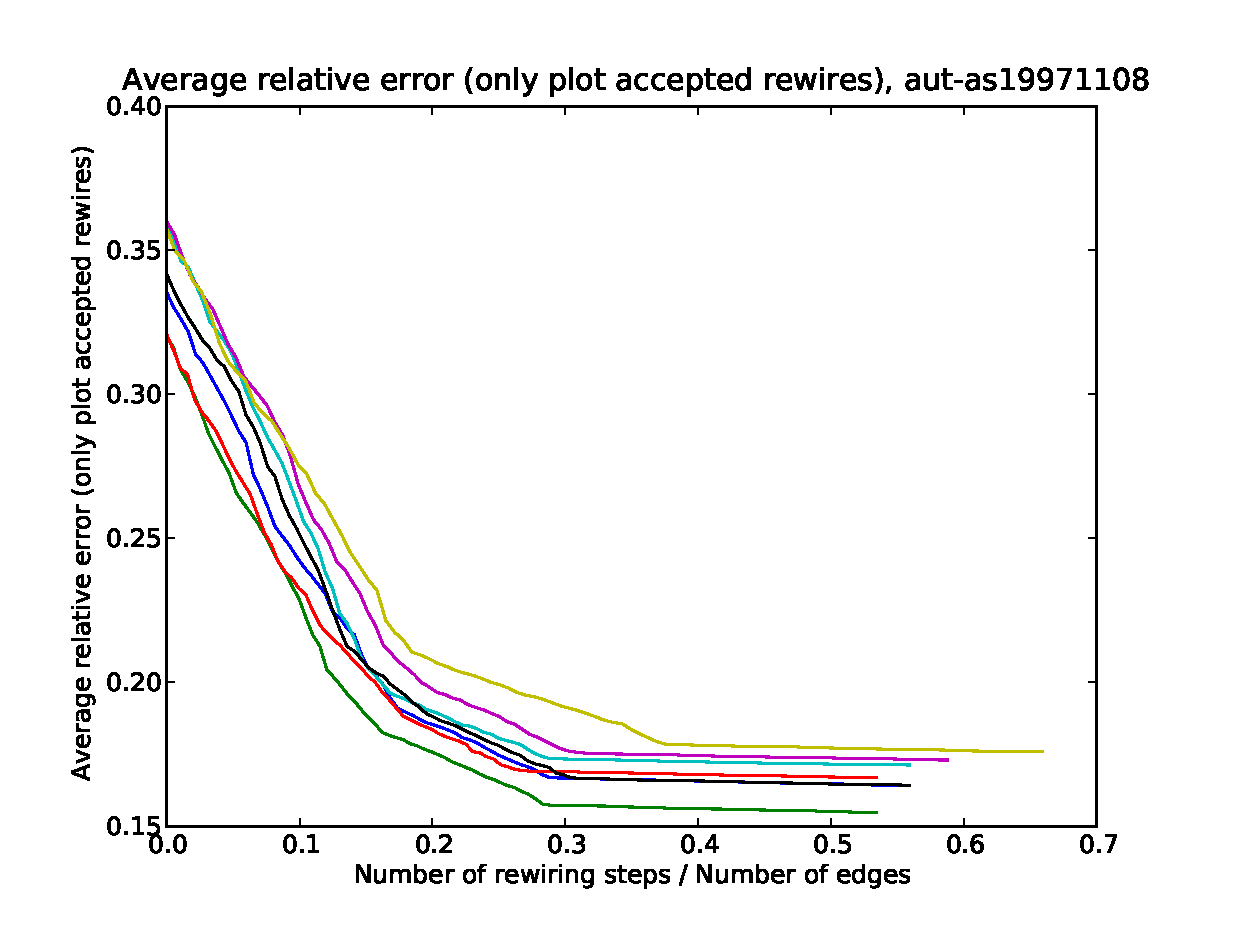
\includegraphics[width=3in]{Figures/acceptedOnly-aut-as19971108.eps}
\caption{Error, network aut-as19971108.  Only plot hill climbing steps that were successful.}
\label{fig:errors-aut-as19971108}
\end{figure}

\begin{figure}[p]
\centering
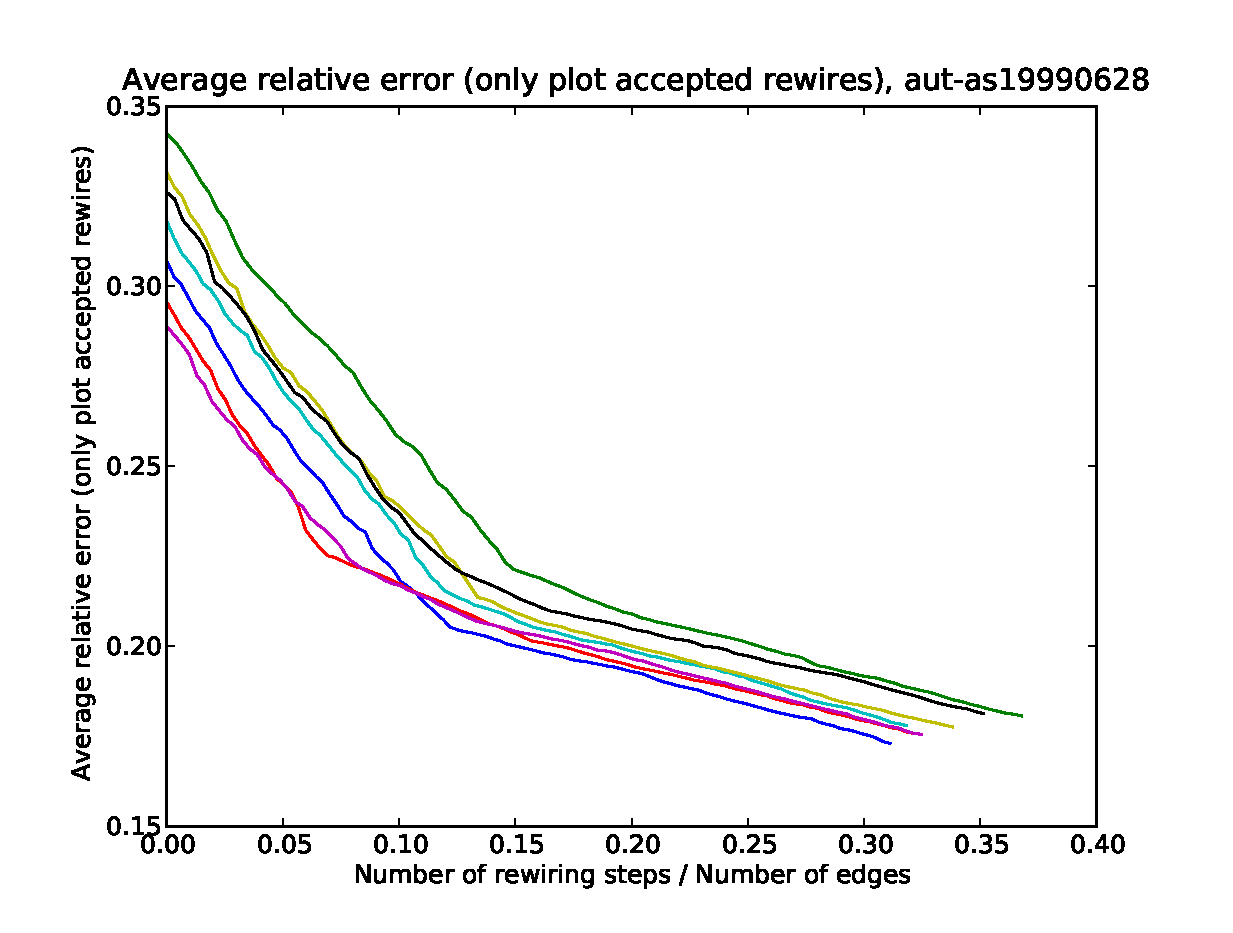
\includegraphics[width=3in]{Figures/acceptedOnly-aut-as19990628.eps}
\caption{Error, network aut-as19990628.  Only plot hill climbing steps that were successful.}
\label{fig:errors-aut-as19990628}
\end{figure}

\begin{figure}[p]
\centering
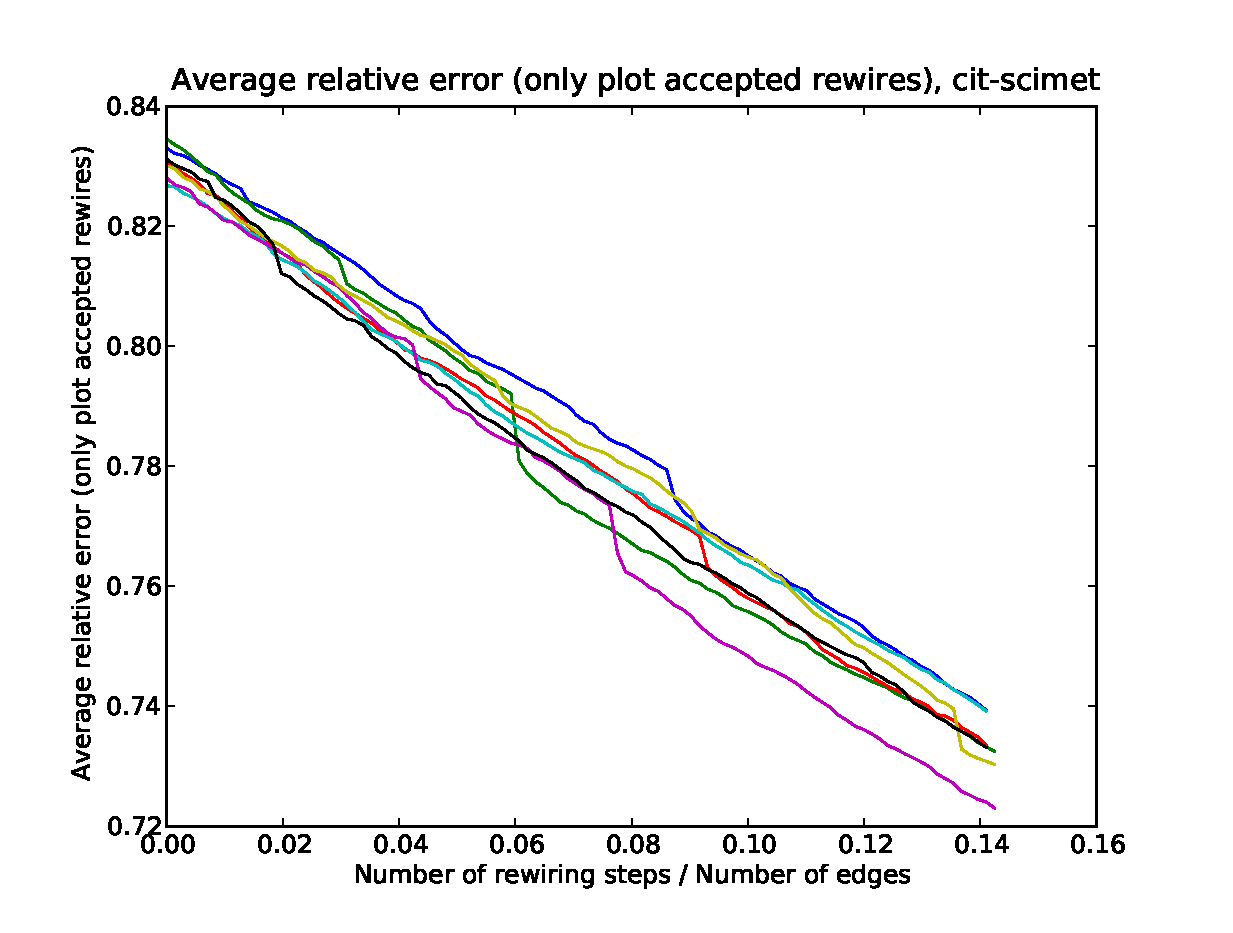
\includegraphics[width=3in]{Figures/acceptedOnly-cit-scimet.eps}
\caption{Error, network cit-scimet.  Only plot hill climbing steps that were successful.}
\label{fig:errors-cit-scimet}
\end{figure}

\begin{figure}[p]
\centering
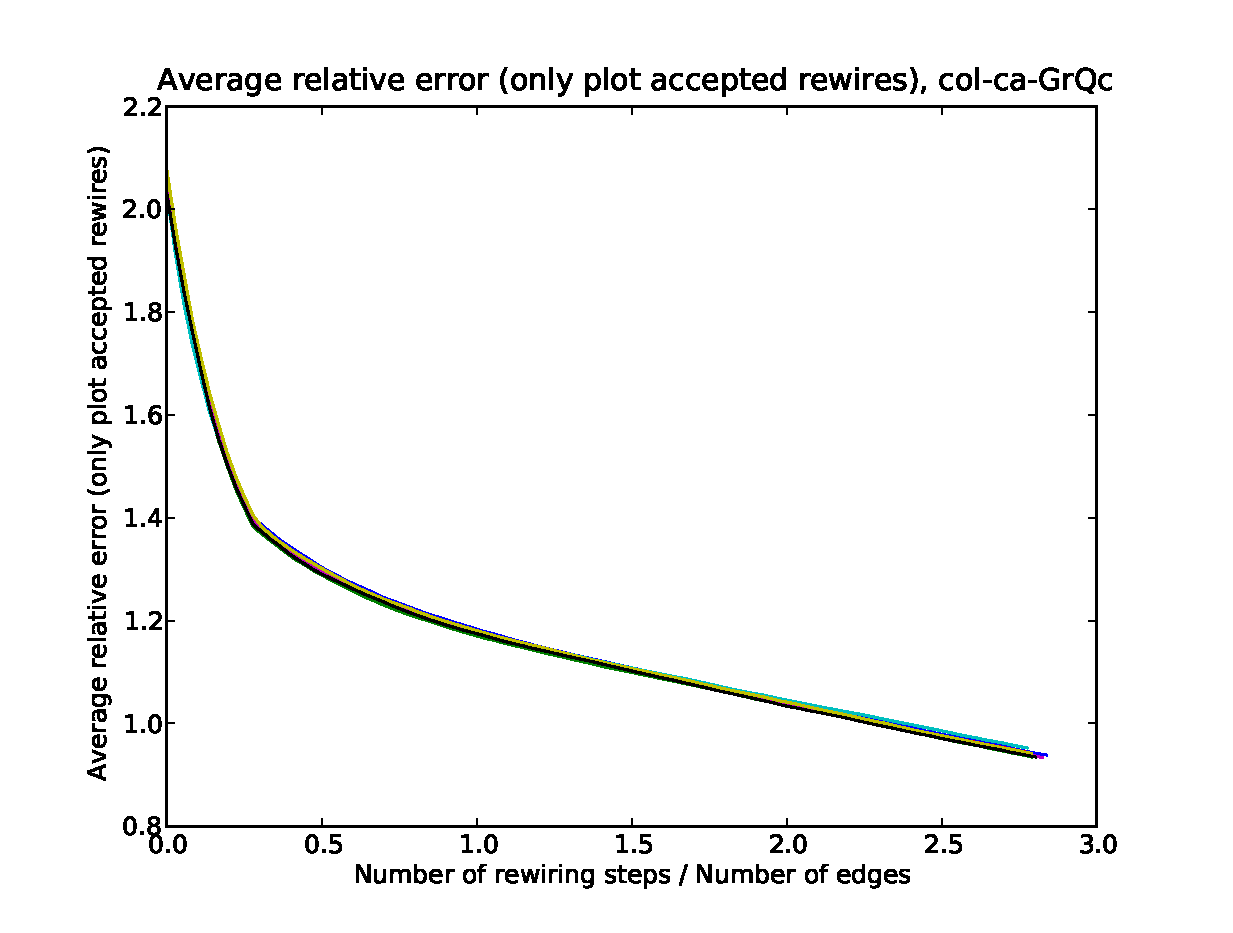
\includegraphics[width=3in]{Figures/acceptedOnly-col-ca-GrQc.eps}
\caption{Error, network col-ca-GrQc.  Only plot hill climbing steps that were successful.}
\label{fig:errors-col-ca-GrQc}
\end{figure}

\begin{figure}[p]
\centering
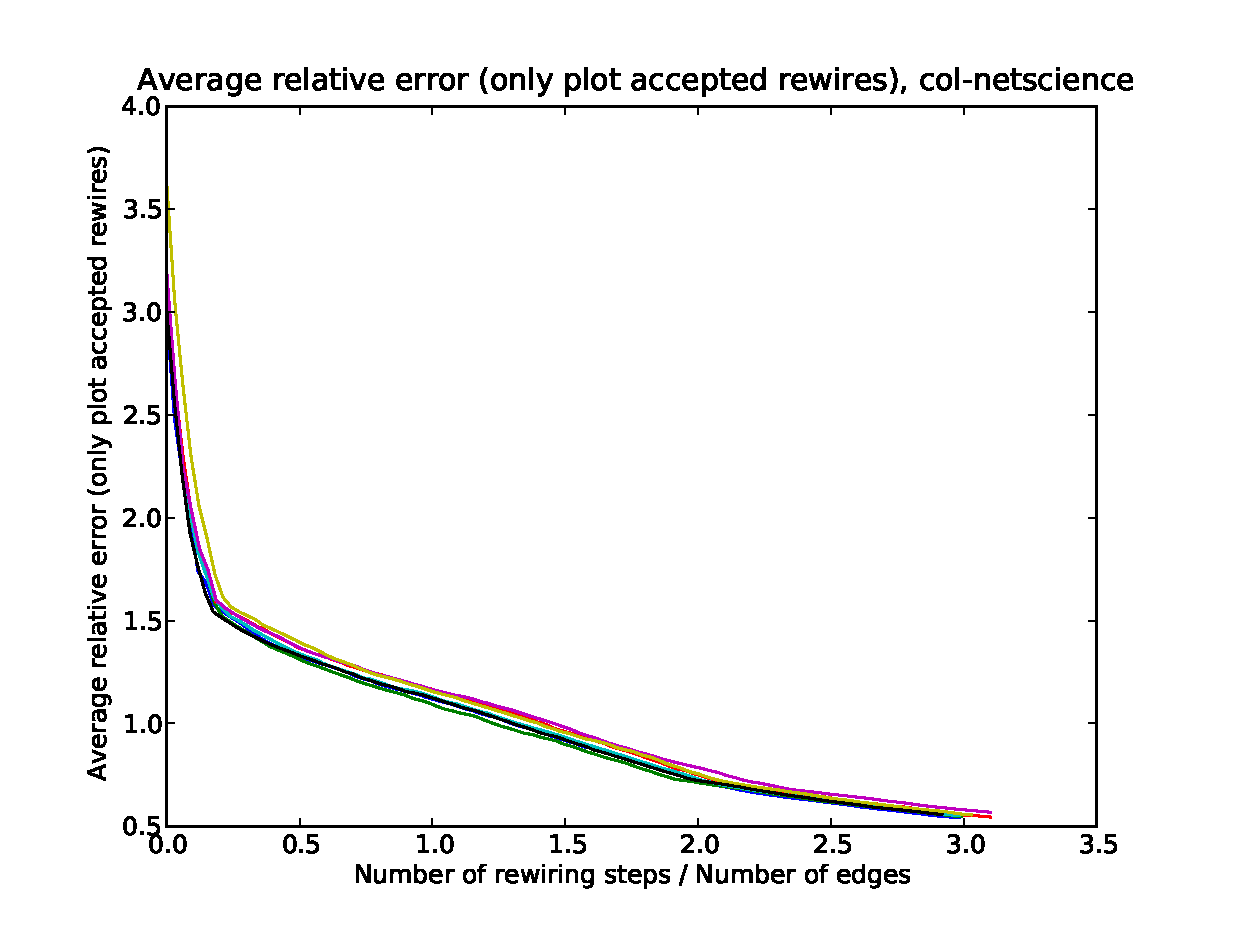
\includegraphics[width=3in]{Figures/acceptedOnly-col-netscience.eps}
\caption{Error, network col-netscience.  Only plot hill climbing steps that were successful.}
\label{fig:errors-col-netscience}
\end{figure}

\begin{figure}[p]
\centering
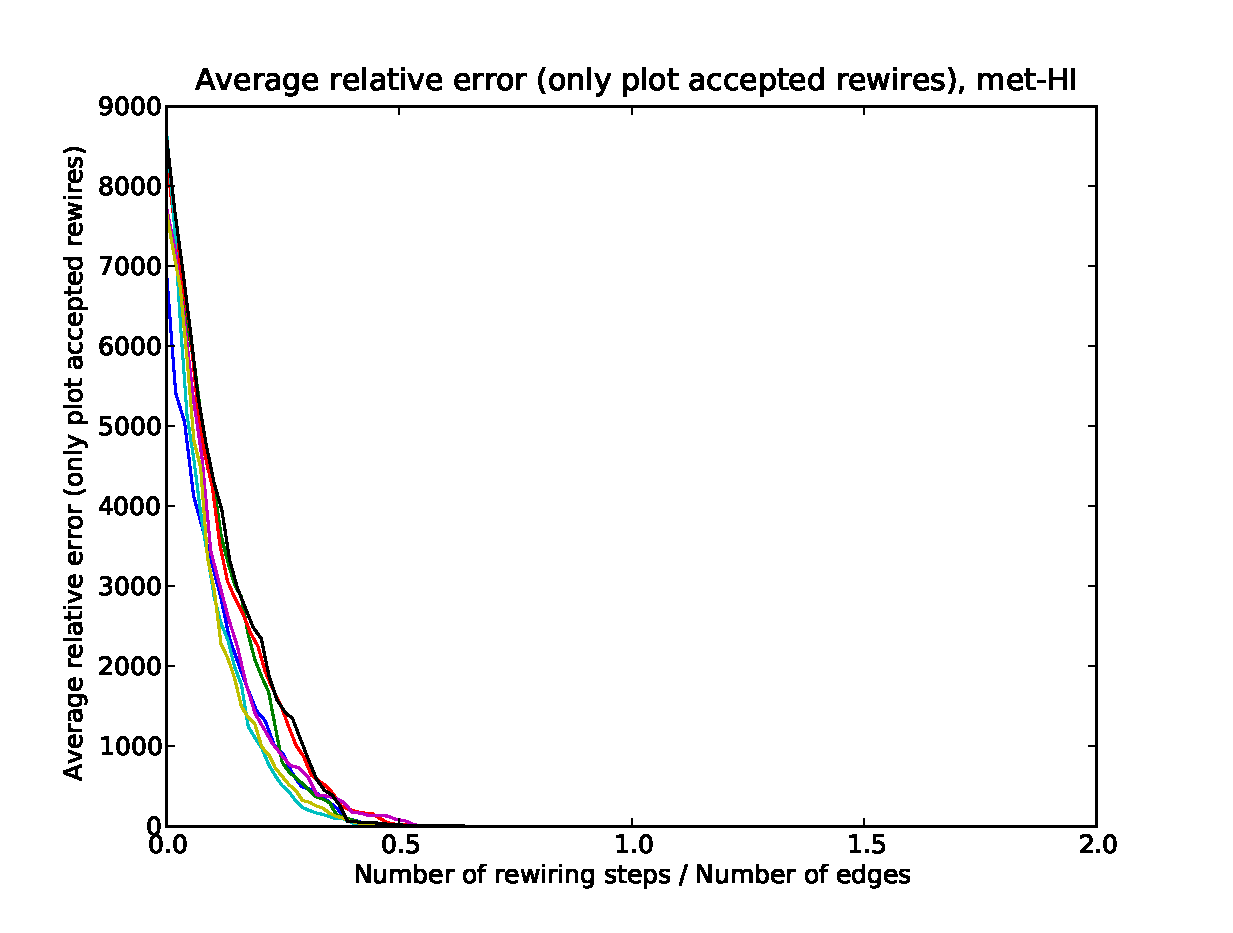
\includegraphics[width=3in]{Figures/acceptedOnly-met-HI.eps}
\caption{Error, network met-HI.  Only plot hill climbing steps that were successful.}
\label{fig:errors-met-HI}
\end{figure}

\begin{figure}[p]
\centering
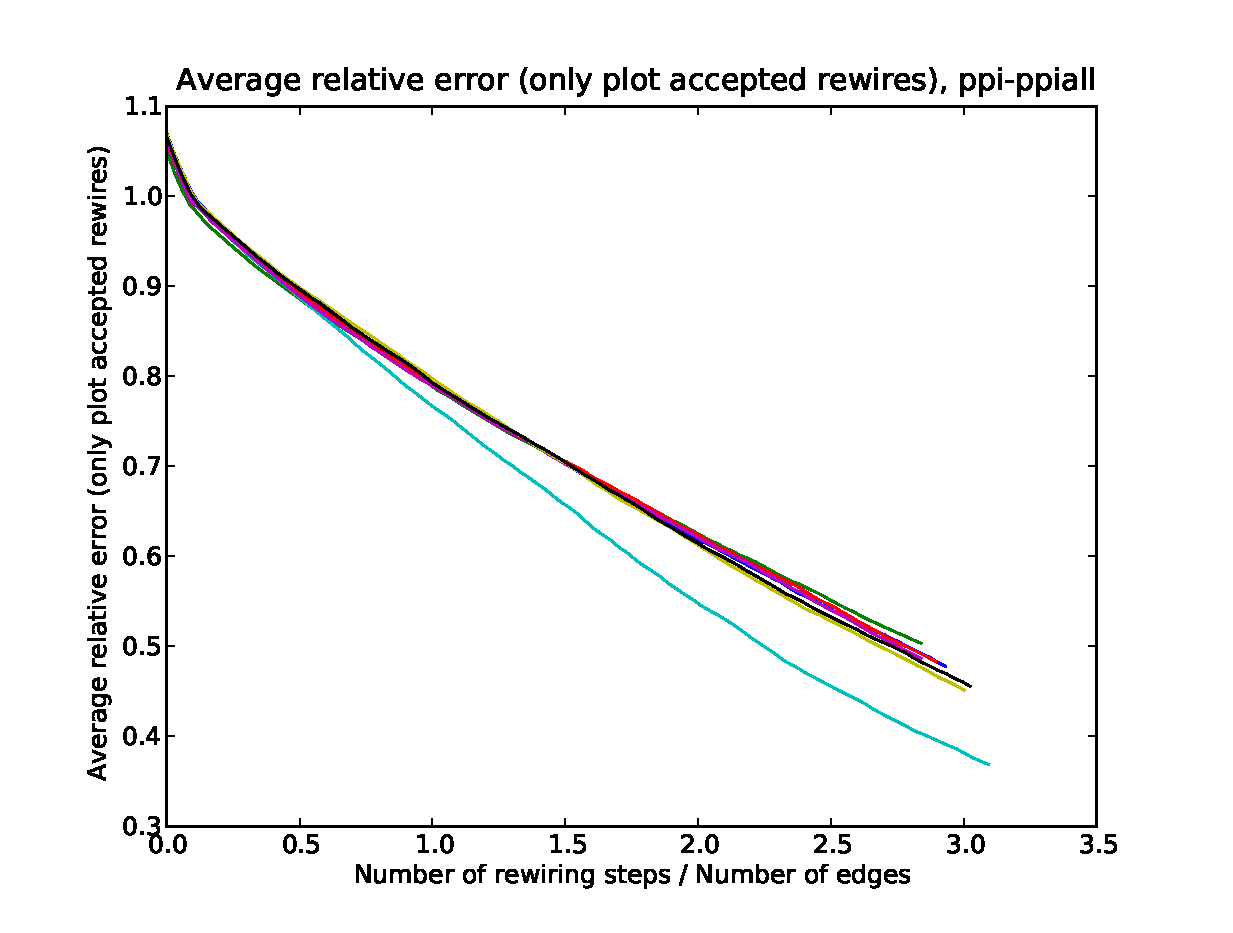
\includegraphics[width=3in]{Figures/acceptedOnly-ppi-ppiall.eps}
\caption{Error, network ppi-ppiall.  Only plot hill climbing steps that were successful.}
\label{fig:errors-ppi-ppiall}
\end{figure}

\begin{figure}[p]
\centering
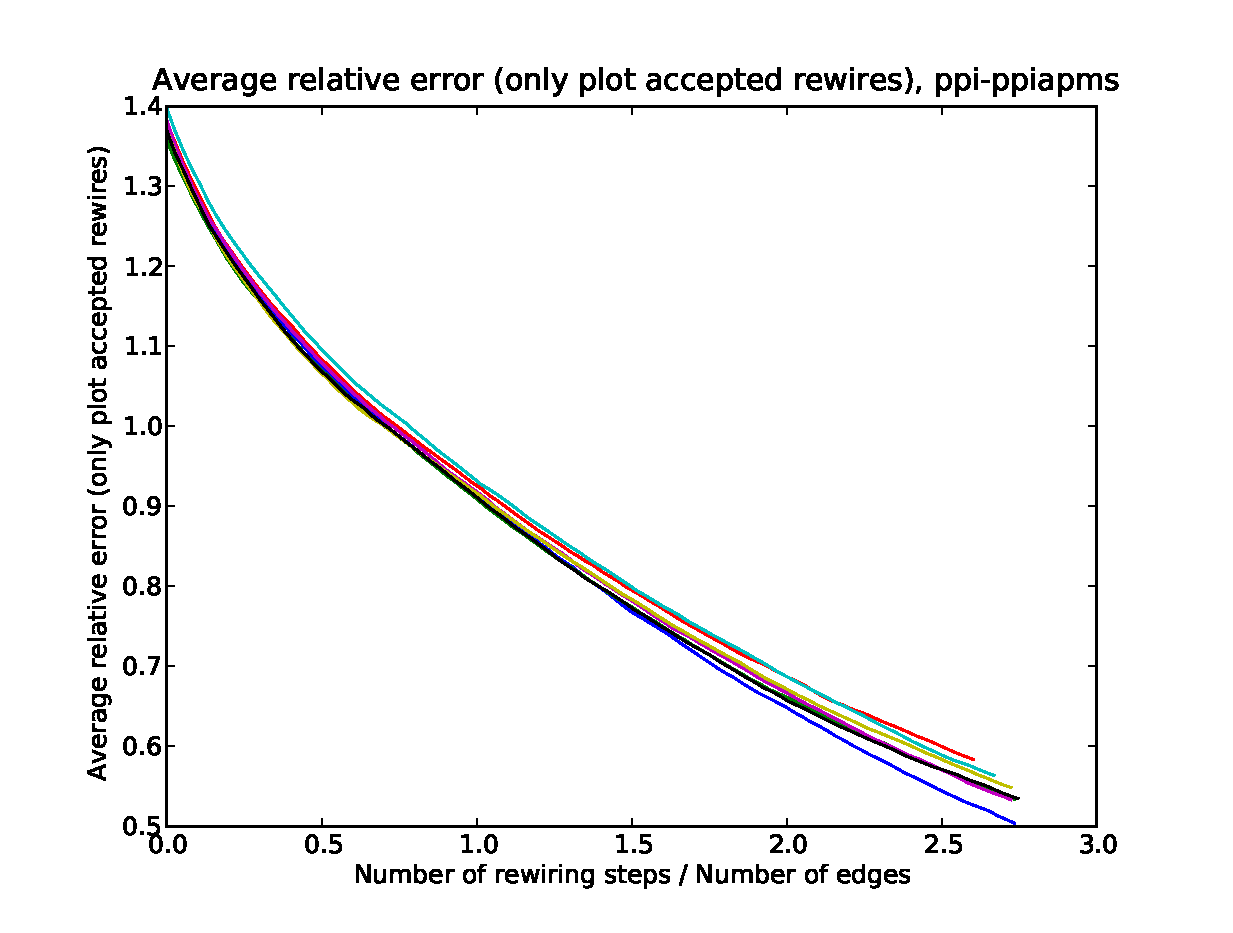
\includegraphics[width=3in]{Figures/acceptedOnly-ppi-ppiapms.eps}
\caption{Error, network ppi-ppiapms.  Only plot hill climbing steps that were successful.}
\label{fig:errors-ppi-ppiapms}
\end{figure}

\begin{figure}[p]
\centering
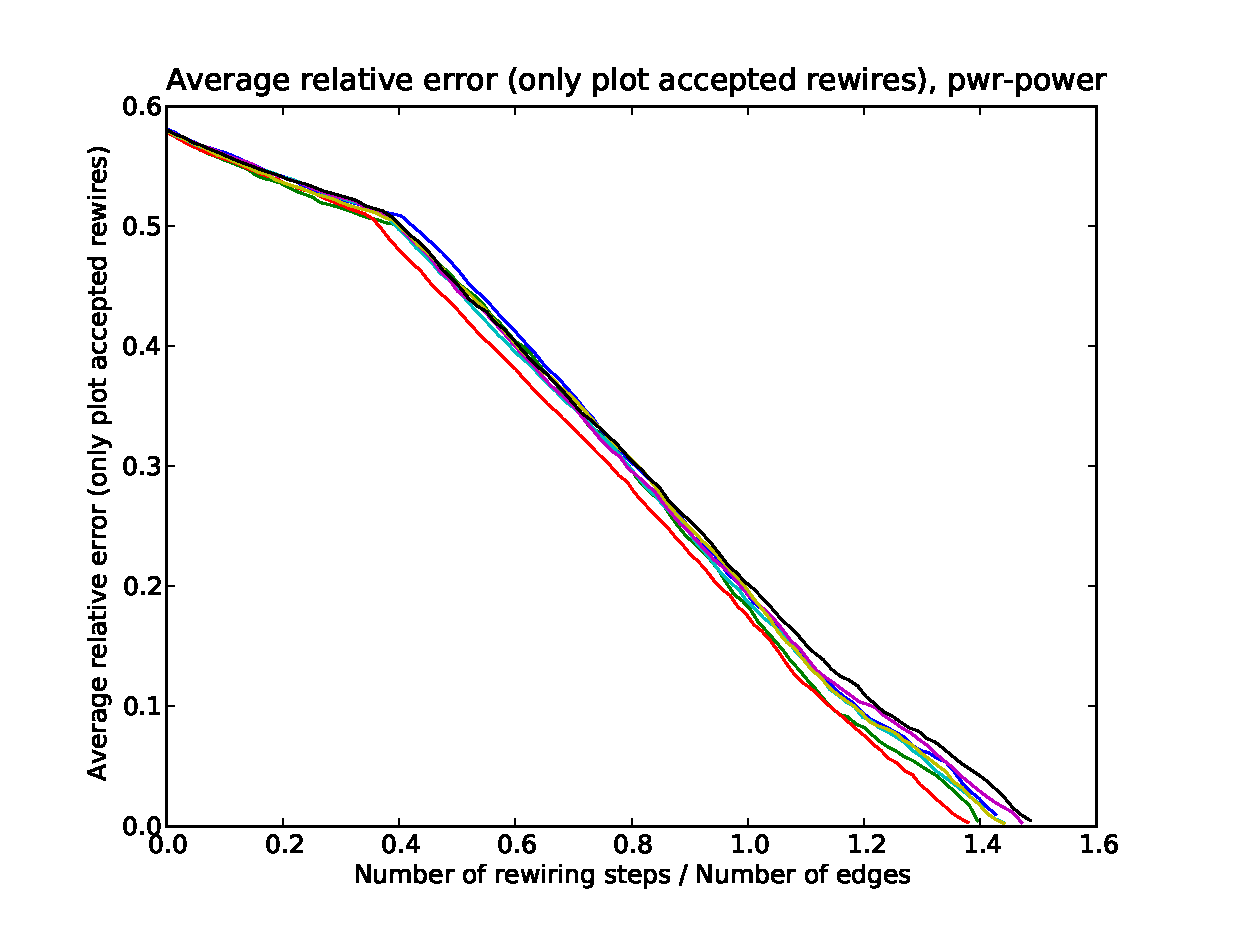
\includegraphics[width=3in]{Figures/acceptedOnly-pwr-power.eps}
\caption{Error, network pwr-power.  Only plot hill climbing steps that were successful.}
\label{fig:errors-pwr-power}
\end{figure}

\begin{figure}[p]
\centering
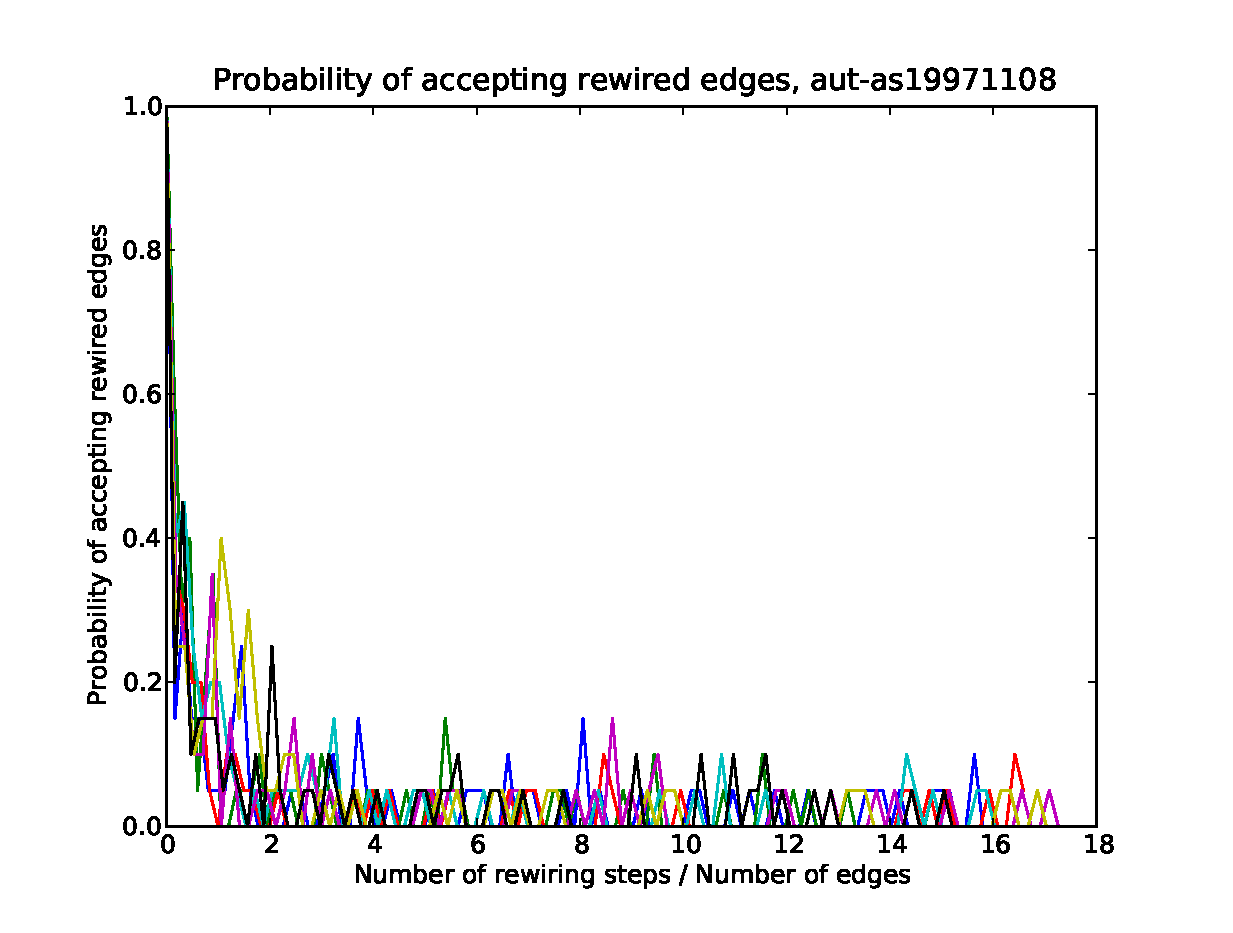
\includegraphics[width=3in]{Figures/Paccept-aut-as19971108.eps}
\caption{Probability of a rewiring step being successful, network aut-as19971108}
\label{fig:Paccept-aut-as19971108}
\end{figure}

\begin{figure}[p]
\centering
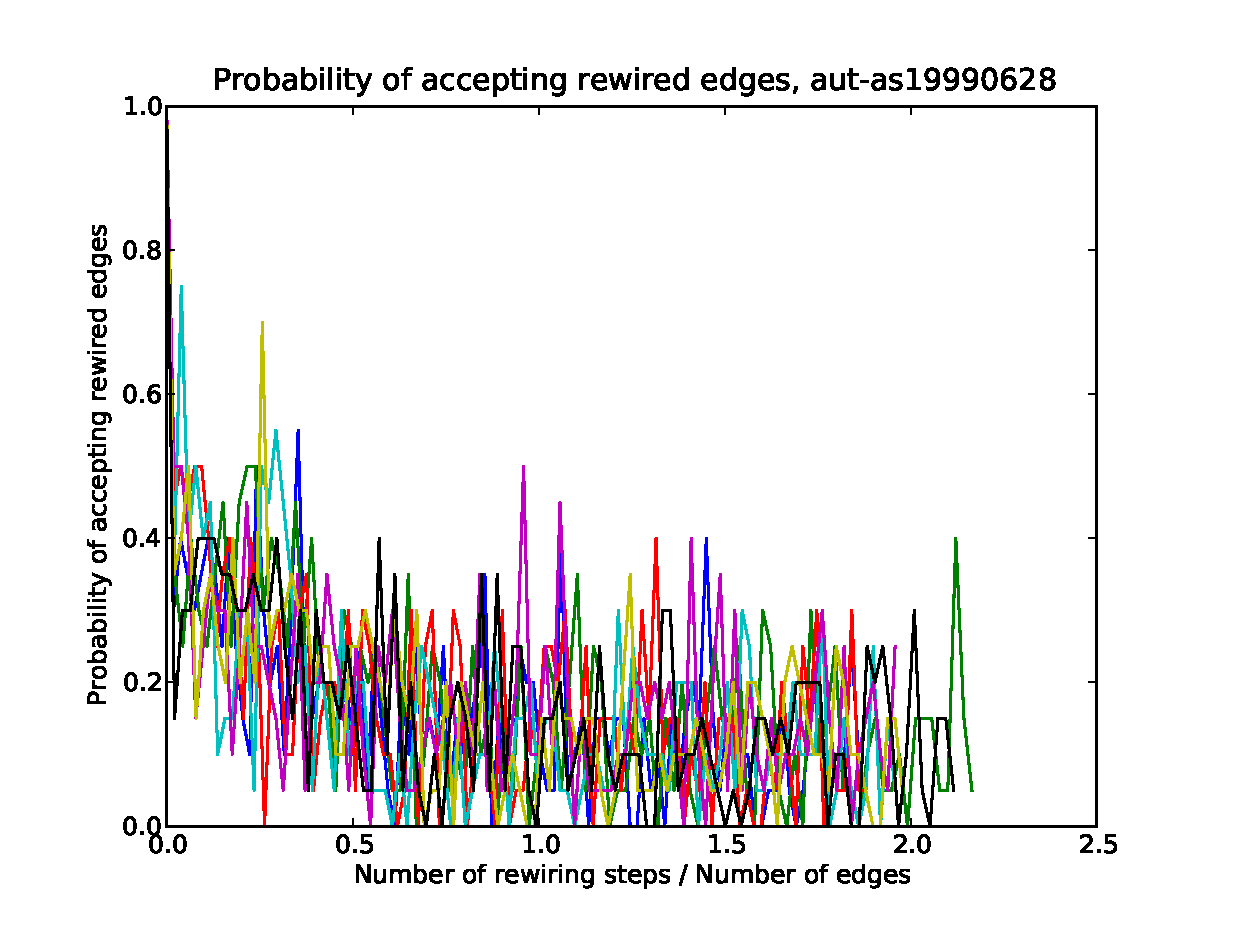
\includegraphics[width=3in]{Figures/Paccept-aut-as19990628.eps}
\caption{Probability of a rewiring step being successful, network aut-as19990628}
\label{fig:Paccept-aut-as19990628}
\end{figure}

\begin{figure}[p]
\centering
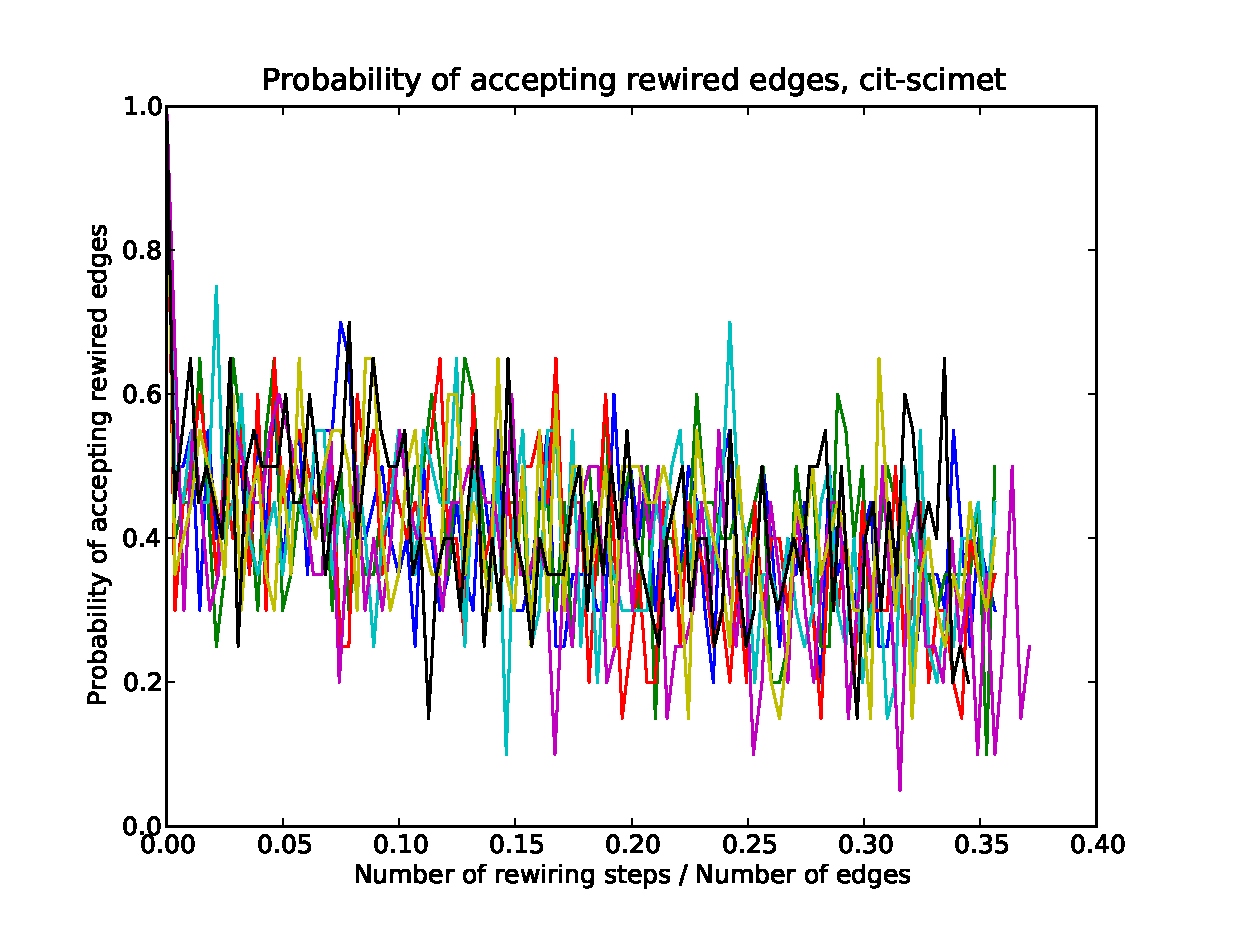
\includegraphics[width=3in]{Figures/Paccept-cit-scimet.eps}
\caption{Probability of a rewiring step being successful, network cit-scimet}
\label{fig:Paccept-cit-scimet}
\end{figure}

\begin{figure}[p]
\centering
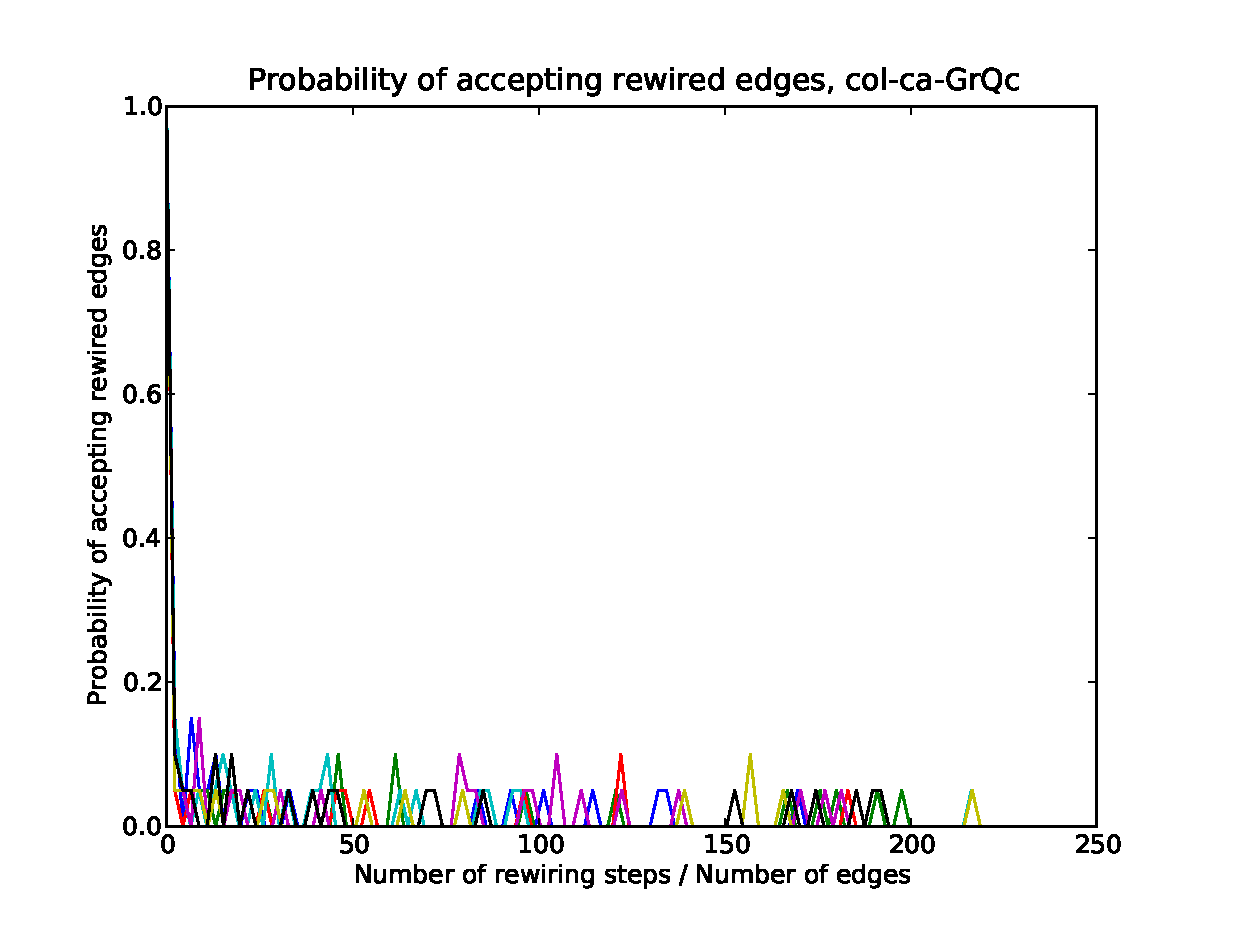
\includegraphics[width=3in]{Figures/Paccept-col-ca-GrQc.eps}
\caption{Probability of a rewiring step being successful, network col-ca-GrQc}
\label{fig:Paccept-col-ca-GrQc}
\end{figure}

\begin{figure}[p]
\centering
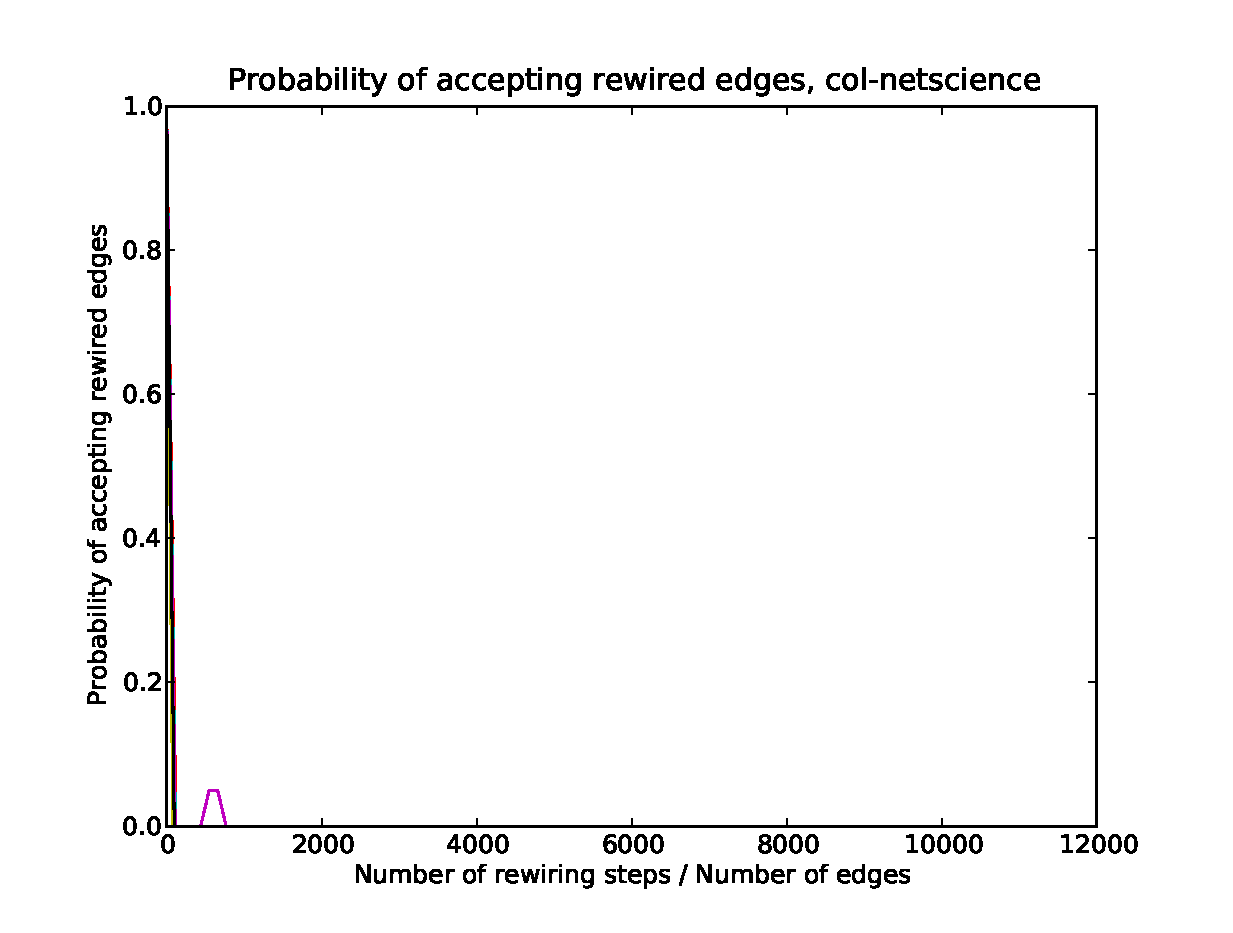
\includegraphics[width=3in]{Figures/Paccept-col-netscience.eps}
\caption{Probability of a rewiring step being successful, network col-netscience}
\label{fig:Paccept-col-netscience}
\end{figure}

\begin{figure}[p]
\centering
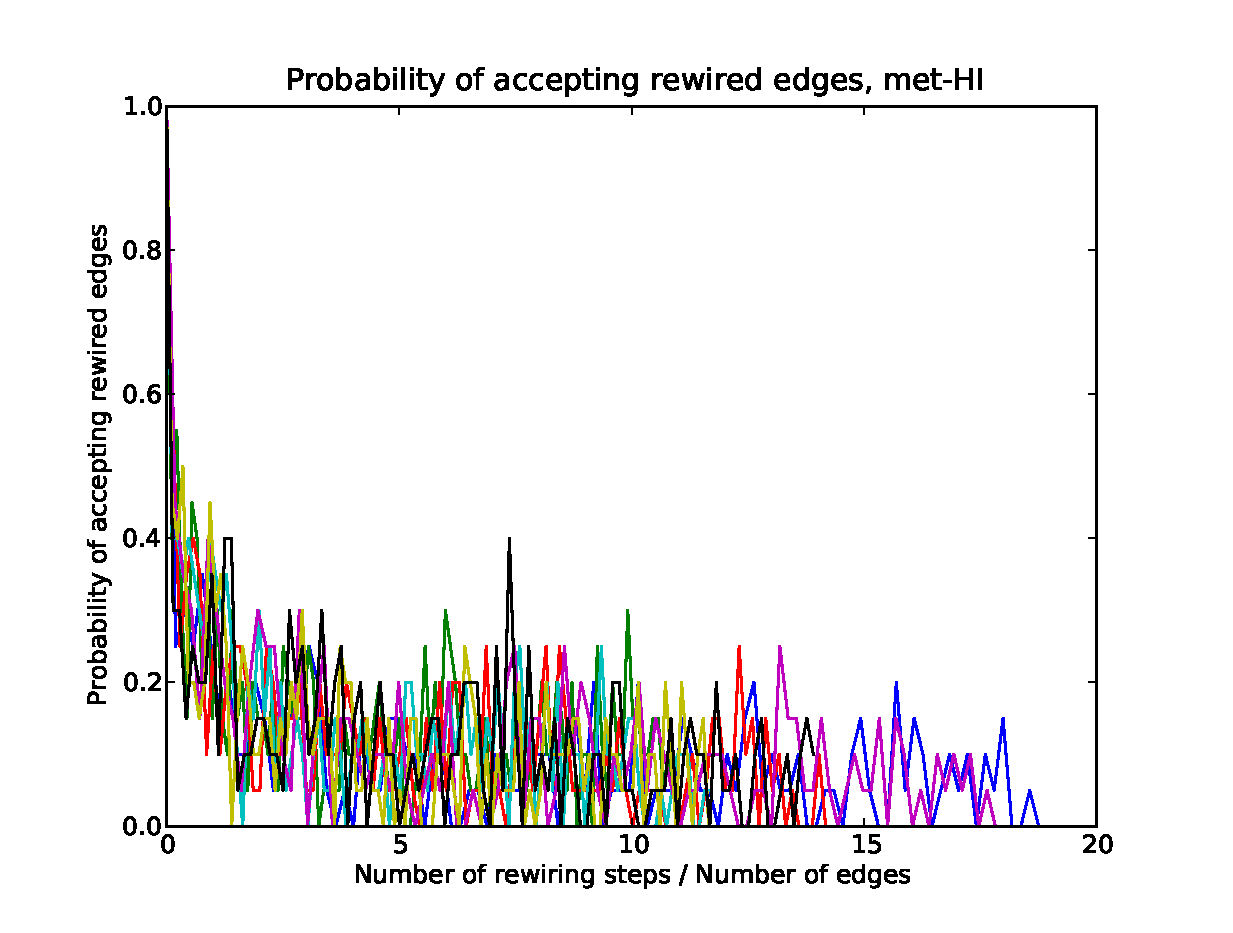
\includegraphics[width=3in]{Figures/Paccept-met-HI.eps}
\caption{Probability of a rewiring step being successful, network met-HI}
\label{fig:Paccept-met-HI}
\end{figure}

\begin{figure}[p]
\centering
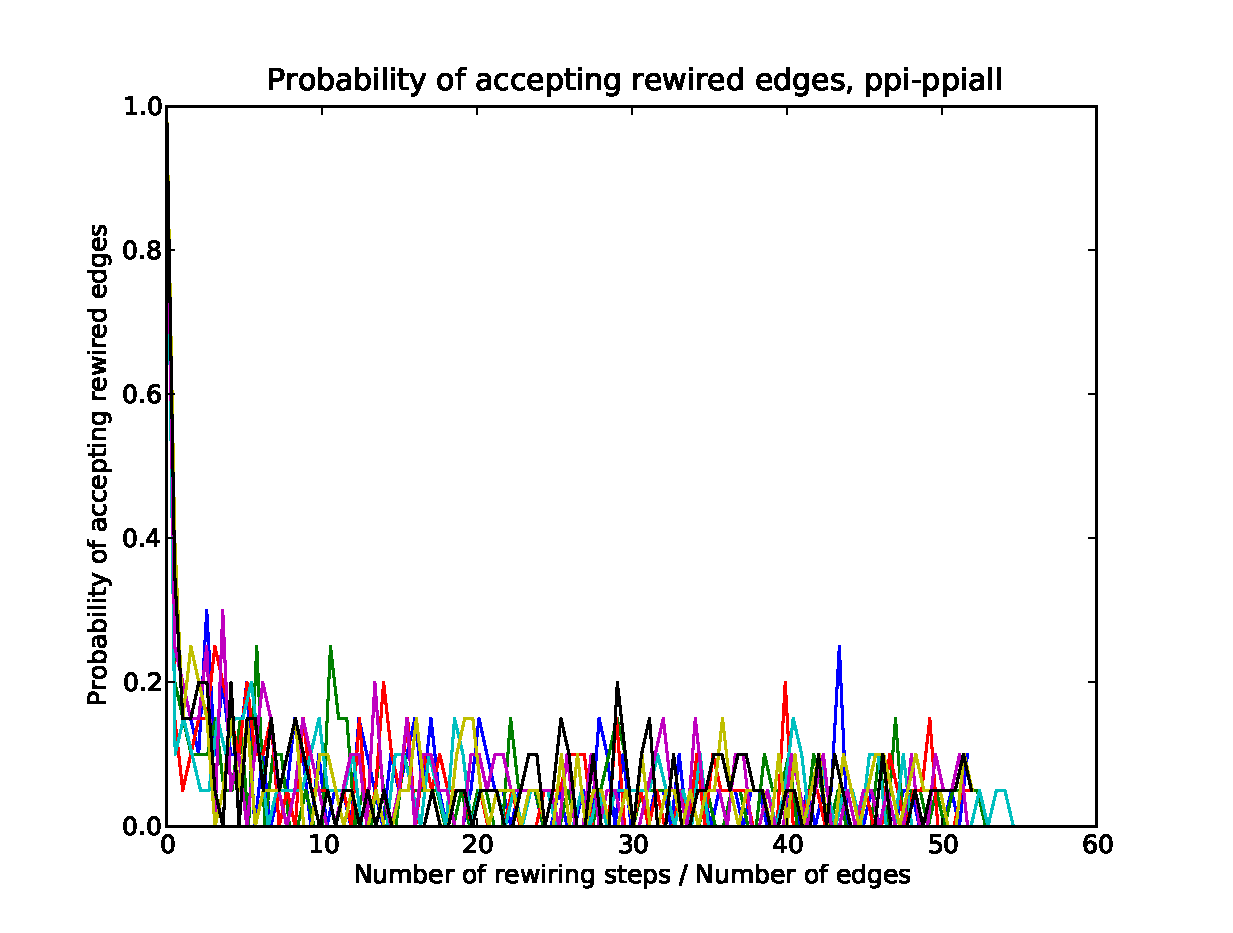
\includegraphics[width=3in]{Figures/Paccept-ppi-ppiall.eps}
\caption{Probability of a rewiring step being successful, network ppi-ppiall}
\label{fig:Paccept-ppi-ppiall}
\end{figure}

\begin{figure}[p]
\centering
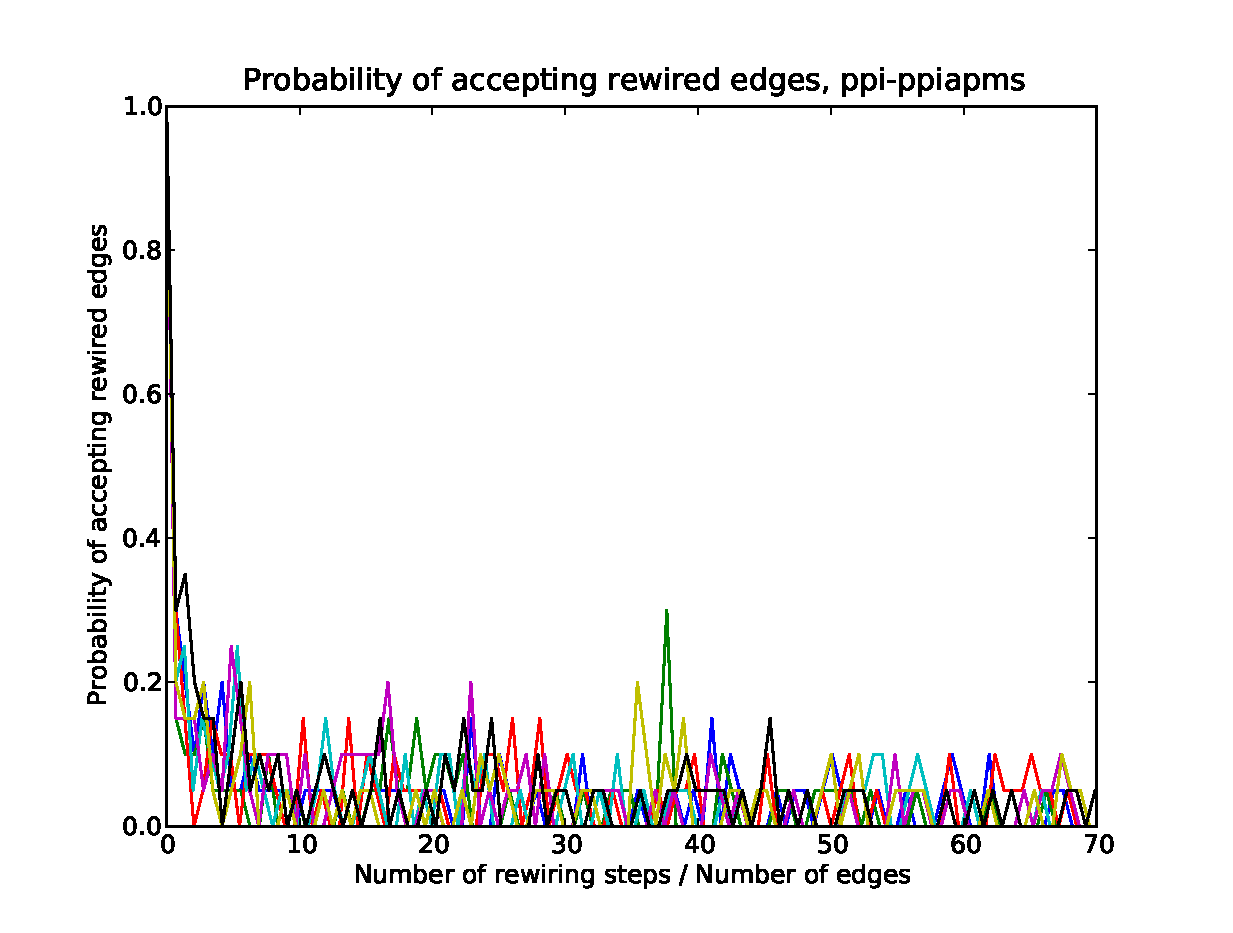
\includegraphics[width=3in]{Figures/Paccept-ppi-ppiapms.eps}
\caption{Probability of a rewiring step being successful, network ppi-ppiapms}
\label{fig:Paccept-ppi-ppiapms}
\end{figure}

\begin{figure}[p]
\centering
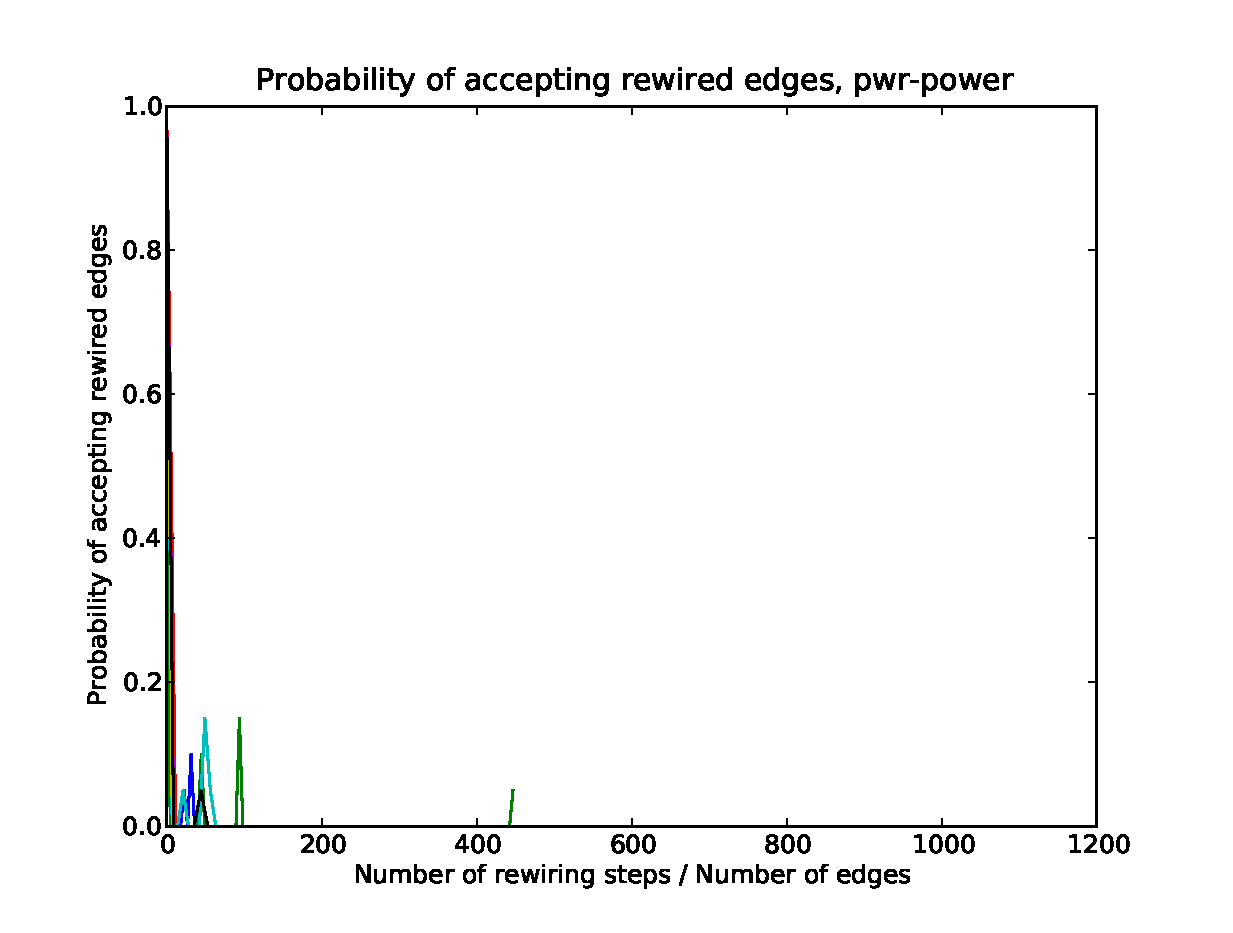
\includegraphics[width=3in]{Figures/Paccept-pwr-power.eps}
\caption{Probability of a rewiring step being successful, network pwr-power}
\label{fig:Paccept-pwr-power}
\end{figure}